%
% gauss.tex -- summarizing the properties of the gauss plane
%
% (c) 2019 Prof Dr Andreas Müller, Hochschule Rapperswil
%
\documentclass[tikz]{standalone}
\usepackage{amsmath}
\usepackage{times}
\usepackage{txfonts}
\usepackage{pgfplots}
\usepackage{csvsimple}
\usetikzlibrary{arrows,intersections}
\begin{document}
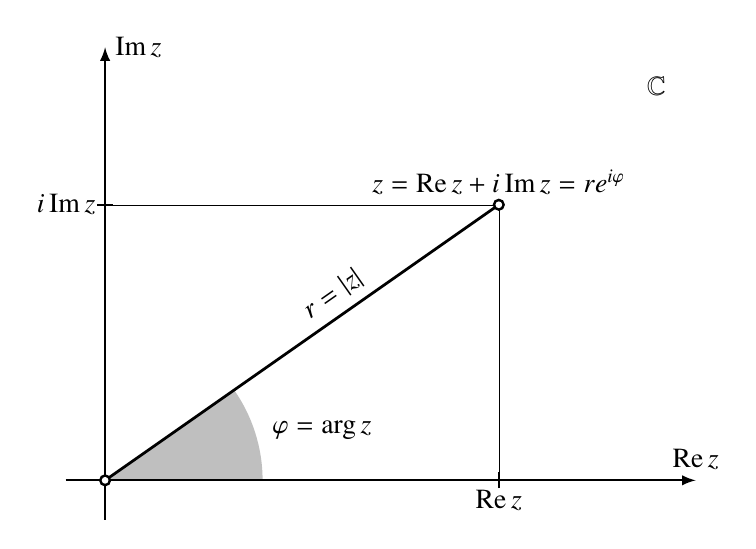
\begin{tikzpicture}[>=latex]
\fill[color=gray!50] (0,0)--(2,0) arc (0:34.992:2)--cycle;

\node at (17.5:2.1) [right] {$\varphi=\operatorname{arg}z$};

\draw[->,line width=0.7pt] (-0.5,0)--(7.5,0)
	coordinate[label={$\operatorname{Re}z$}];
\draw[->,line width=0.7pt] (0,-0.5)--(0,5.5)
	coordinate[label={right:$\operatorname{Im}z$}];
\node at (7,5) {$\mathbb C$};
\def\punkt#1{
\draw[fill] #1 circle[radius=2pt];
\draw[fill,color=white] #1 circle[radius=1pt];
}
\draw[line width=1pt] (0,0)--(5,3.5);
\draw[line width=0.1pt] (5,0)--(5,3.5);
\draw[line width=0.1pt] (0,3.5)--(5,3.5);
\punkt{(0,0)}
\punkt{(5,3.5)}
\node at (5,3.5) [above]
	{$z = \operatorname{Re}z+i\operatorname{Im}z=re^{i\varphi}$};
\draw[line width=0.7pt] (5,-0.1)--(5,0.1);
\draw[line width=0.7pt] (-0.1,3.5)--(0.1,3.5);
\node at (5,0) [below] {$\operatorname{Re}z$};
\node at (0,3.5) [left] {$i\operatorname{Im}z$};
\node at ({0.7*5},{0.7*3.5}) [rotate=35,above left] {$r=|z|$};
\end{tikzpicture}
\end{document}

